\noindent
\begin{minipage}[t]{0.26\textwidth}
  % Cột lề trái: Dóng hàng đỉnh Hình 17 chính xác với đoạn "Ta cần xác định..."
  \vspace*{48pt}
  \noindent
  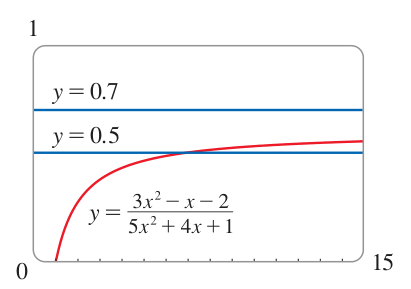
\includegraphics[width=\textwidth]{images/p0171_fig1.png}
  
  \vspace{5pt}
  \noindent
  {\small\textbf{\textsf{HÌNH 17}}}
\end{minipage}%
\hfill
\begin{minipage}[t]{0.70\textwidth}
  \noindent
  \textbf{\textsf{\color{stewartcyan}LỜI GIẢI}}\hspace{1em}Ta viết lại bất đẳng thức đã cho dưới dạng
  \begin{equation*}
    0.5 < \frac{3x^2 - x - 2}{5x^2 + 4x + 1} < 0.7
  \end{equation*}
  Ta cần xác định các giá trị của $x$ sao cho đường cong đã cho nằm giữa các đường thẳng nằm ngang $y = 0.5$ và $y = 0.7$. Do đó, ta vẽ đồ thị đường cong và các đường thẳng này trong Hình~17. Sau đó, ta sử dụng đồ thị để ước lượng rằng đường cong cắt đường thẳng $y = 0.5$ khi $x \approx 6.7$. Về phía bên phải của giá trị này, có vẻ như đường cong luôn nằm giữa hai đường thẳng $y = 0.5$ và $y = 0.7$. Làm tròn lên để đảm bảo an toàn, ta có thể nói rằng
  \begin{equation*}
    \text{nếu}\quad x > 7 \quad\text{thì}\quad \left| \frac{3x^2 - x - 2}{5x^2 + 4x + 1} - 0.6 \right| < 0.1
  \end{equation*}
  Nói cách khác, với $\varepsilon = 0.1$ ta có thể chọn $N = 7$ (hoặc bất kỳ số nào lớn hơn) trong Định nghĩa~7.\hspace*{\fill}{\color{stewartcyan}\rule{1.15ex}{1.15ex}}

  \vspace{1.5em}
  \noindent
  \textbf{\textsf{\color{stewartcyan}VÍ DỤ 14}}\hspace{1em}Sử dụng Định nghĩa~7 để chứng minh rằng $\lim\limits_{x \to \infty} \dfrac{1}{x} = 0$.

  \vspace{0.6em}
  \noindent
  \textbf{\textsf{\color{stewartcyan}LỜI GIẢI}}\hspace{1em}Cho trước $\varepsilon > 0$, ta muốn tìm $N$ sao cho
  \begin{equation*}
    \text{nếu}\quad x > N \quad\text{thì}\quad \left| \frac{1}{x} - 0 \right| < \varepsilon
  \end{equation*}
  Khi tính giới hạn, ta có thể giả định rằng $x > 0$. Khi đó $1/x < \varepsilon \iff x > 1/\varepsilon$. Ta hãy chọn $N = 1/\varepsilon$. Khi đó
  \begin{equation*}
    \text{nếu}\quad x > N = \frac{1}{\varepsilon} \quad\text{thì}\quad \left| \frac{1}{x} - 0 \right| = \frac{1}{x} < \varepsilon
  \end{equation*}
  Do đó, theo Định nghĩa~7,
  \begin{equation*}
    \lim_{x \to \infty} \frac{1}{x} = 0
  \end{equation*}
  Hình~18 minh họa cho phép chứng minh bằng cách thể hiện một vài giá trị của $\varepsilon$ và các giá trị tương ứng của $N$.
\end{minipage}

\vspace{1.5em}
\noindent
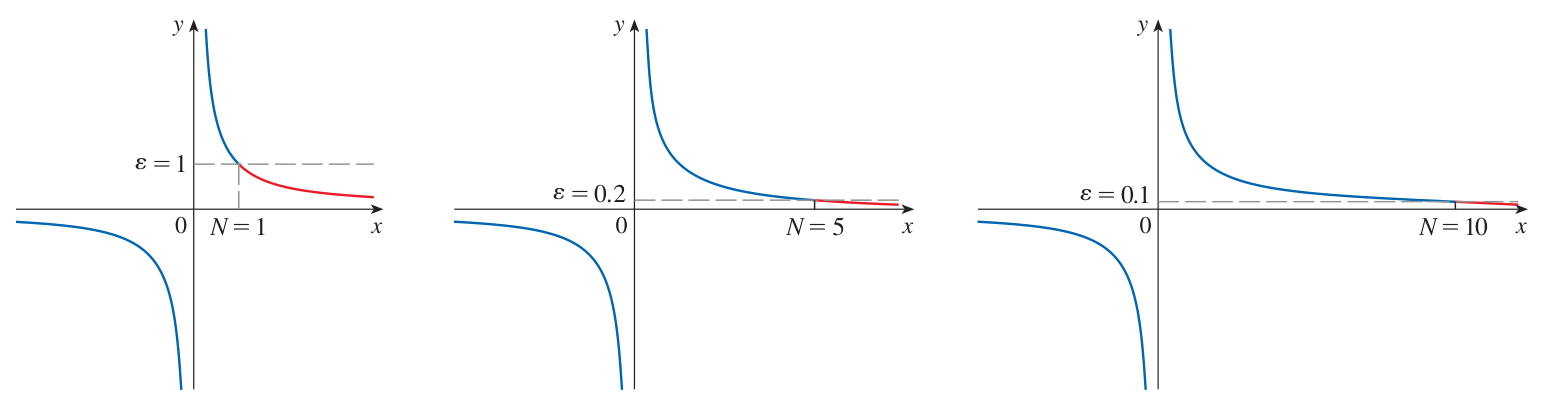
\includegraphics[width=\textwidth]{images/p0171_fig2.png}

\vspace{5pt}
\noindent
{\small\textbf{\textsf{HÌNH 18}}}\hfill{\color{stewartcyan}\rule{1.15ex}{1.15ex}}
